\begin{frame}
    \frametitle{Network Architecture}
    
    \begin{columns}[T]
        \begin{column}{0.7\textwidth}
            \begin{alertblock}{Model}
                \begin{itemize}
                    \item $\num{4}$ Dense Layers with Dropout
                    \item Trainable parameters: $\num{85254}$
                    \item Loss function: categorical crossentropy
                    \item Optimizer: adam
                \end{itemize}    
            \end{alertblock}
            \begin{alertblock}{Training}
                \begin{itemize}
                    \item Early stopping: Stops training when the validation loss function no longer improves
                    \item Reduce learning rate: Decreases learning rate if validation loss function stagnates \\
                    \to better convergence
                    \item Train the model using the training data with the defined set of hyperparameters.
                \end{itemize}  
            \end{alertblock}
        \end{column}
        \begin{column}{0.3\textwidth}
            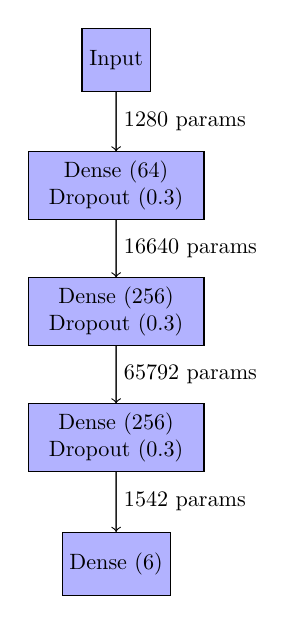
\begin{tikzpicture}[
                scale=0.8, every node/.style={scale=0.8},
                layer/.style={rectangle,draw=black,fill=blue!30,minimum size=1cm},
                sum/.style={circle,draw=black,fill=yellow!30},
            ]
            
            % Define nodes
            \node[layer] (L0) at (0,0) {Input};
            \node[layer] (L1) at (0,-2) {\begin{tabular}{c} Dense (64) \\ Dropout (0.3) \end{tabular}};
            \node[layer] (L2) at (0,-4) {\begin{tabular}{c} Dense (256) \\ Dropout (0.3) \end{tabular}};
            \node[layer] (L3) at (0,-6) {\begin{tabular}{c} Dense (256) \\ Dropout (0.3) \end{tabular}};
            \node[layer] (L4) at (0,-8) {Dense (6)};
        
            % Draw connections
            \draw[->] (L0) -- (L1);
            \draw[->] (L1) -- (L2);
            \draw[->] (L2) -- (L3);
            \draw[->] (L3) -- (L4);
            
            % Draw parameter counts
            \draw (L0) -- (L1) node[midway,right] {1280 params};
            \draw (L1) -- (L2) node[midway,right] {16640 params};
            \draw (L2) -- (L3) node[midway,right] {65792 params};
            \draw (L3) -- (L4) node[midway,right] {1542 params};
            
            \end{tikzpicture}
        \end{column}
    \end{columns}

\end{frame}
